\documentclass[11pt, a4paper]{article}
\usepackage{pdfpages}
\usepackage{parallel}
\usepackage[T2A]{fontenc}
\usepackage{ucs}
\usepackage[utf8x]{inputenc}
\usepackage[polish,english,russian]{babel}
\usepackage{hyperref}
\usepackage{rotating}
\usepackage[inner=2cm,top=1.8cm,outer=2cm,bottom=2.3cm,nohead]{geometry}
\usepackage{listings}
\usepackage{graphicx}
\usepackage{wrapfig}
\usepackage{longtable}
\usepackage{indentfirst}
\usepackage{array}
\usepackage{tikzsymbols}
\usepackage{soul}
\usepackage[ruled,vlined]{algorithm2e}
%\counterwithout{figure}{section} 

\usepackage{url}
\makeatletter
\g@addto@macro{\UrlBreaks}{\UrlOrds}
\makeatother

\newcolumntype{P}[1]{>{\raggedright\arraybackslash}p{#1}}
\frenchspacing
\usepackage{fixltx2e} %text sub- and superscripts
\usepackage{icomma} % коскі ў матэматычным рэжыме
\PreloadUnicodePage{4}

\newcommand{\longpage}{\enlargethispage{\baselineskip}}
\newcommand{\shortpage}{\enlargethispage{-\baselineskip}}

\def\switchlang#1{\expandafter\csname switchlang#1\endcsname}
\def\switchlangbe{
\let\saverefname=\refname%
\def\refname{Літаратура}%
\def\figurename{Іл.}%
}
\def\switchlangen{
\let\saverefname=\refname%
\def\refname{References}%
\def\figurename{Fig.}%
}
\def\switchlangru{
\let\saverefname=\refname%
\let\savefigurename=\figurename%
\def\refname{Литература}%
\def\figurename{Рис.}%
}

\hyphenation{admi-ni-stra-tive}
\hyphenation{ex-pe-ri-ence}
\hyphenation{fle-xi-bi-li-ty}
\hyphenation{Py-thon}
\hyphenation{ma-the-ma-ti-cal}
\hyphenation{re-ported}
\hyphenation{imp-le-menta-tions}
\hyphenation{pro-vides}
\hyphenation{en-gi-neering}
\hyphenation{com-pa-ti-bi-li-ty}
\hyphenation{im-pos-sible}
\hyphenation{desk-top}
\hyphenation{elec-tro-nic}
\hyphenation{com-pa-ny}
\hyphenation{de-ve-lop-ment}
\hyphenation{de-ve-loping}
\hyphenation{de-ve-lop}
\hyphenation{da-ta-ba-se}
\hyphenation{plat-forms}
\hyphenation{or-ga-ni-za-tion}
\hyphenation{pro-gramming}
\hyphenation{in-stru-ments}
\hyphenation{Li-nux}
\hyphenation{sour-ce}
\hyphenation{en-vi-ron-ment}
\hyphenation{Te-le-pathy}
\hyphenation{Li-nux-ov-ka}
\hyphenation{Open-BSD}
\hyphenation{Free-BSD}
\hyphenation{men-ti-on-ed}
\hyphenation{app-li-ca-tion}

\def\progref!#1!{\texttt{#1}}
\renewcommand{\arraystretch}{2} %Іначай формулы ў матрыцы зліпаюцца з лініямі
\usepackage{array}

\def\interview #1 (#2), #3, #4, #5\par{

\section[#1, #3, #4]{#1 -- #3, #4}
\def\qname{LVEE}
\def\aname{#1}
\def\q ##1\par{{\noindent \bf \qname: ##1 }\par}
\def\a{{\noindent \bf \aname: } \def\qname{L}\def\aname{#2}}
}

\def\interview* #1 (#2), #3, #4, #5\par{

\section*{#1\\{\small\rm #3, #4. #5}}
\ifx\ParallelWhichBox\undefined%
    \addcontentsline{toc}{section}{#1, #3, #4}%
\else%
\ifnum\ParallelWhichBox=0%
    \addcontentsline{toc}{section}{#1, #3, #4}%
\fi\fi%

\def\qname{LVEE}
\def\aname{#1}
\def\q ##1\par{{\noindent \bf \qname: ##1 }\par}
\def\a{{\noindent \bf \aname: } \def\qname{L}\def\aname{#2}}
}

\newcommand{\interviewfooter}[1]{
\vskip 1em
\noindent \textit{#1}
}

\switchlang{en}
\begin{document}

\title{1987 "--- MicroSpeed FastTRAP trackball}
\date{}
\maketitle
\selectlanguage{english}
The FastTRAP device from MicroSpeed, released in 1987, is a trackball with three buttons, as well as an additional wheel, thanks to which it can generate coordinates not along two, but along three coordinate axes - \textit{x}, \textit{y} and \textit{z} - that is, it supports one more coordinate plane than a mouse or tablet (figure \ref{fig:FastTRAPPic}). The additional axis was designed primarily for users of CAD solid modeling, since the simultaneous change in three coordinate axes at once can reduce the time required to rotate an object or projection in the viewport.

\begin{figure}[h]
   \centering
    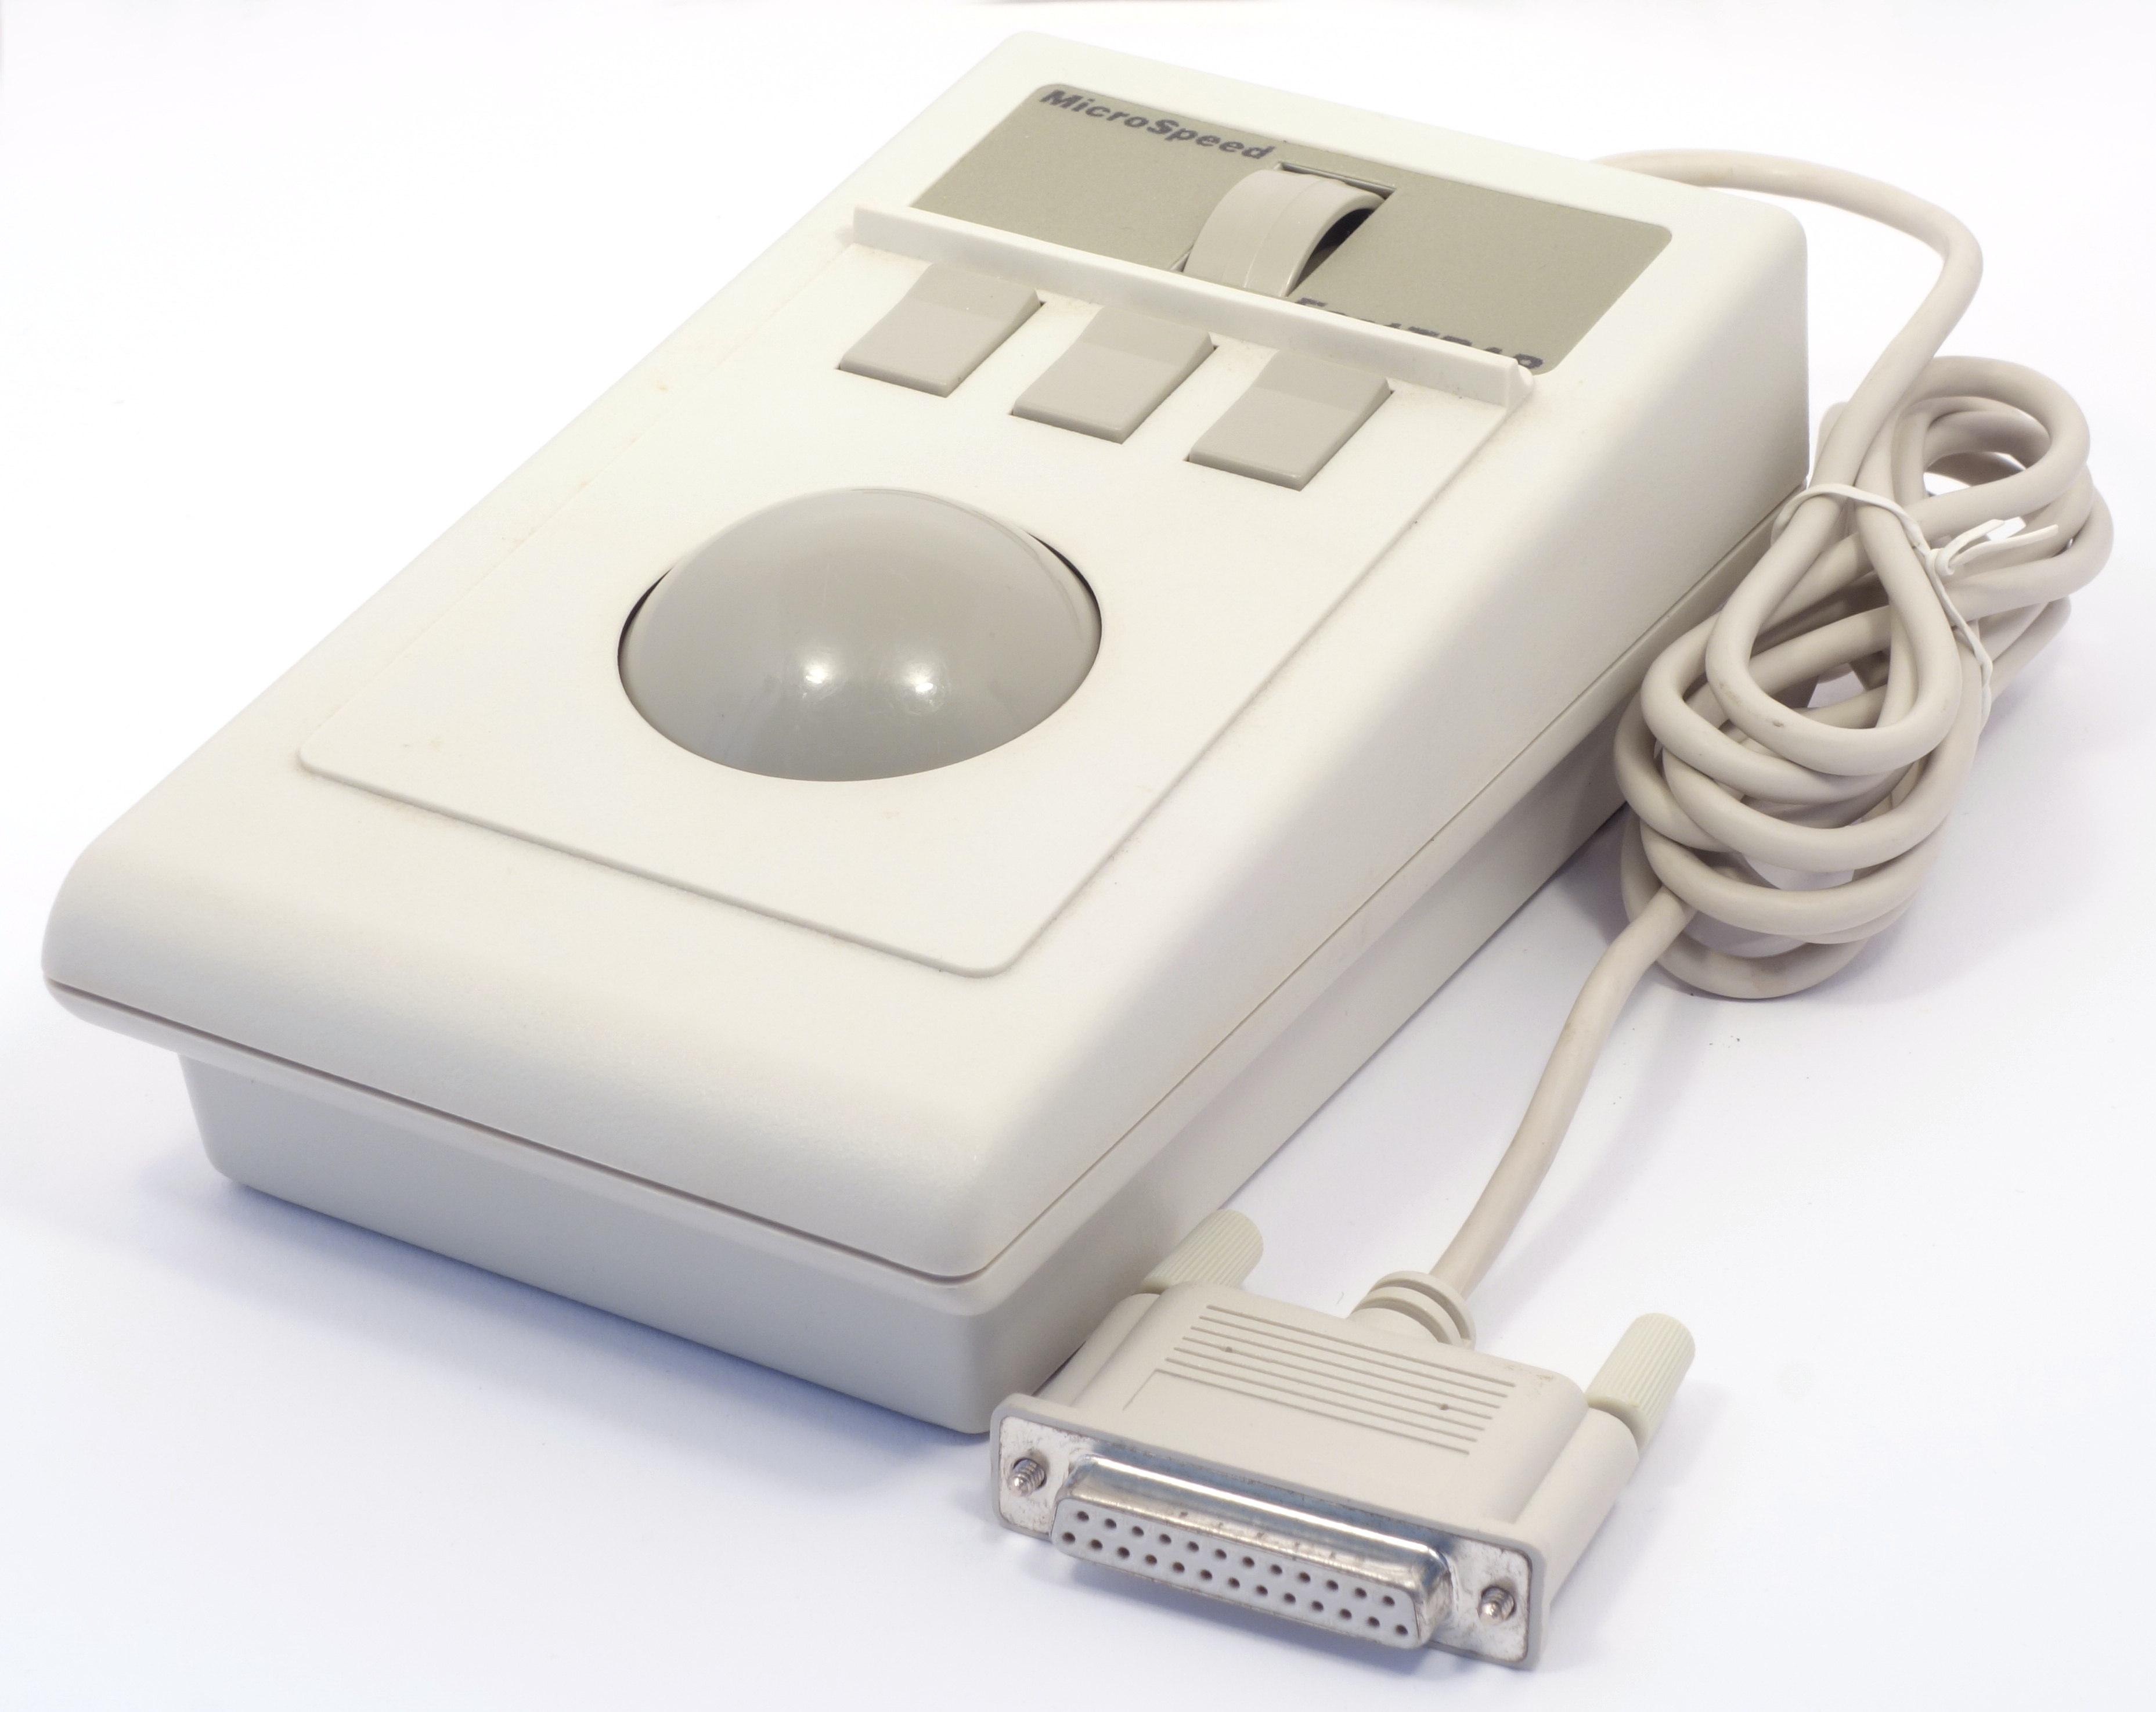
\includegraphics[scale=0.3]{1987_microspeed_fasttrap/pic_15.jpg}
    \caption{MicroSpeed FastTRAP trackball}
    \label{fig:FastTRAPPic}
\end{figure}

The \textit{z} axis is controlled by turning the wheel; however, at the time this device was released, the concept of a scroll wheel did not yet exist, so the software does not allow it to be used for scrolling in graphics or text programs.

\begin{figure}[h]
    \centering
    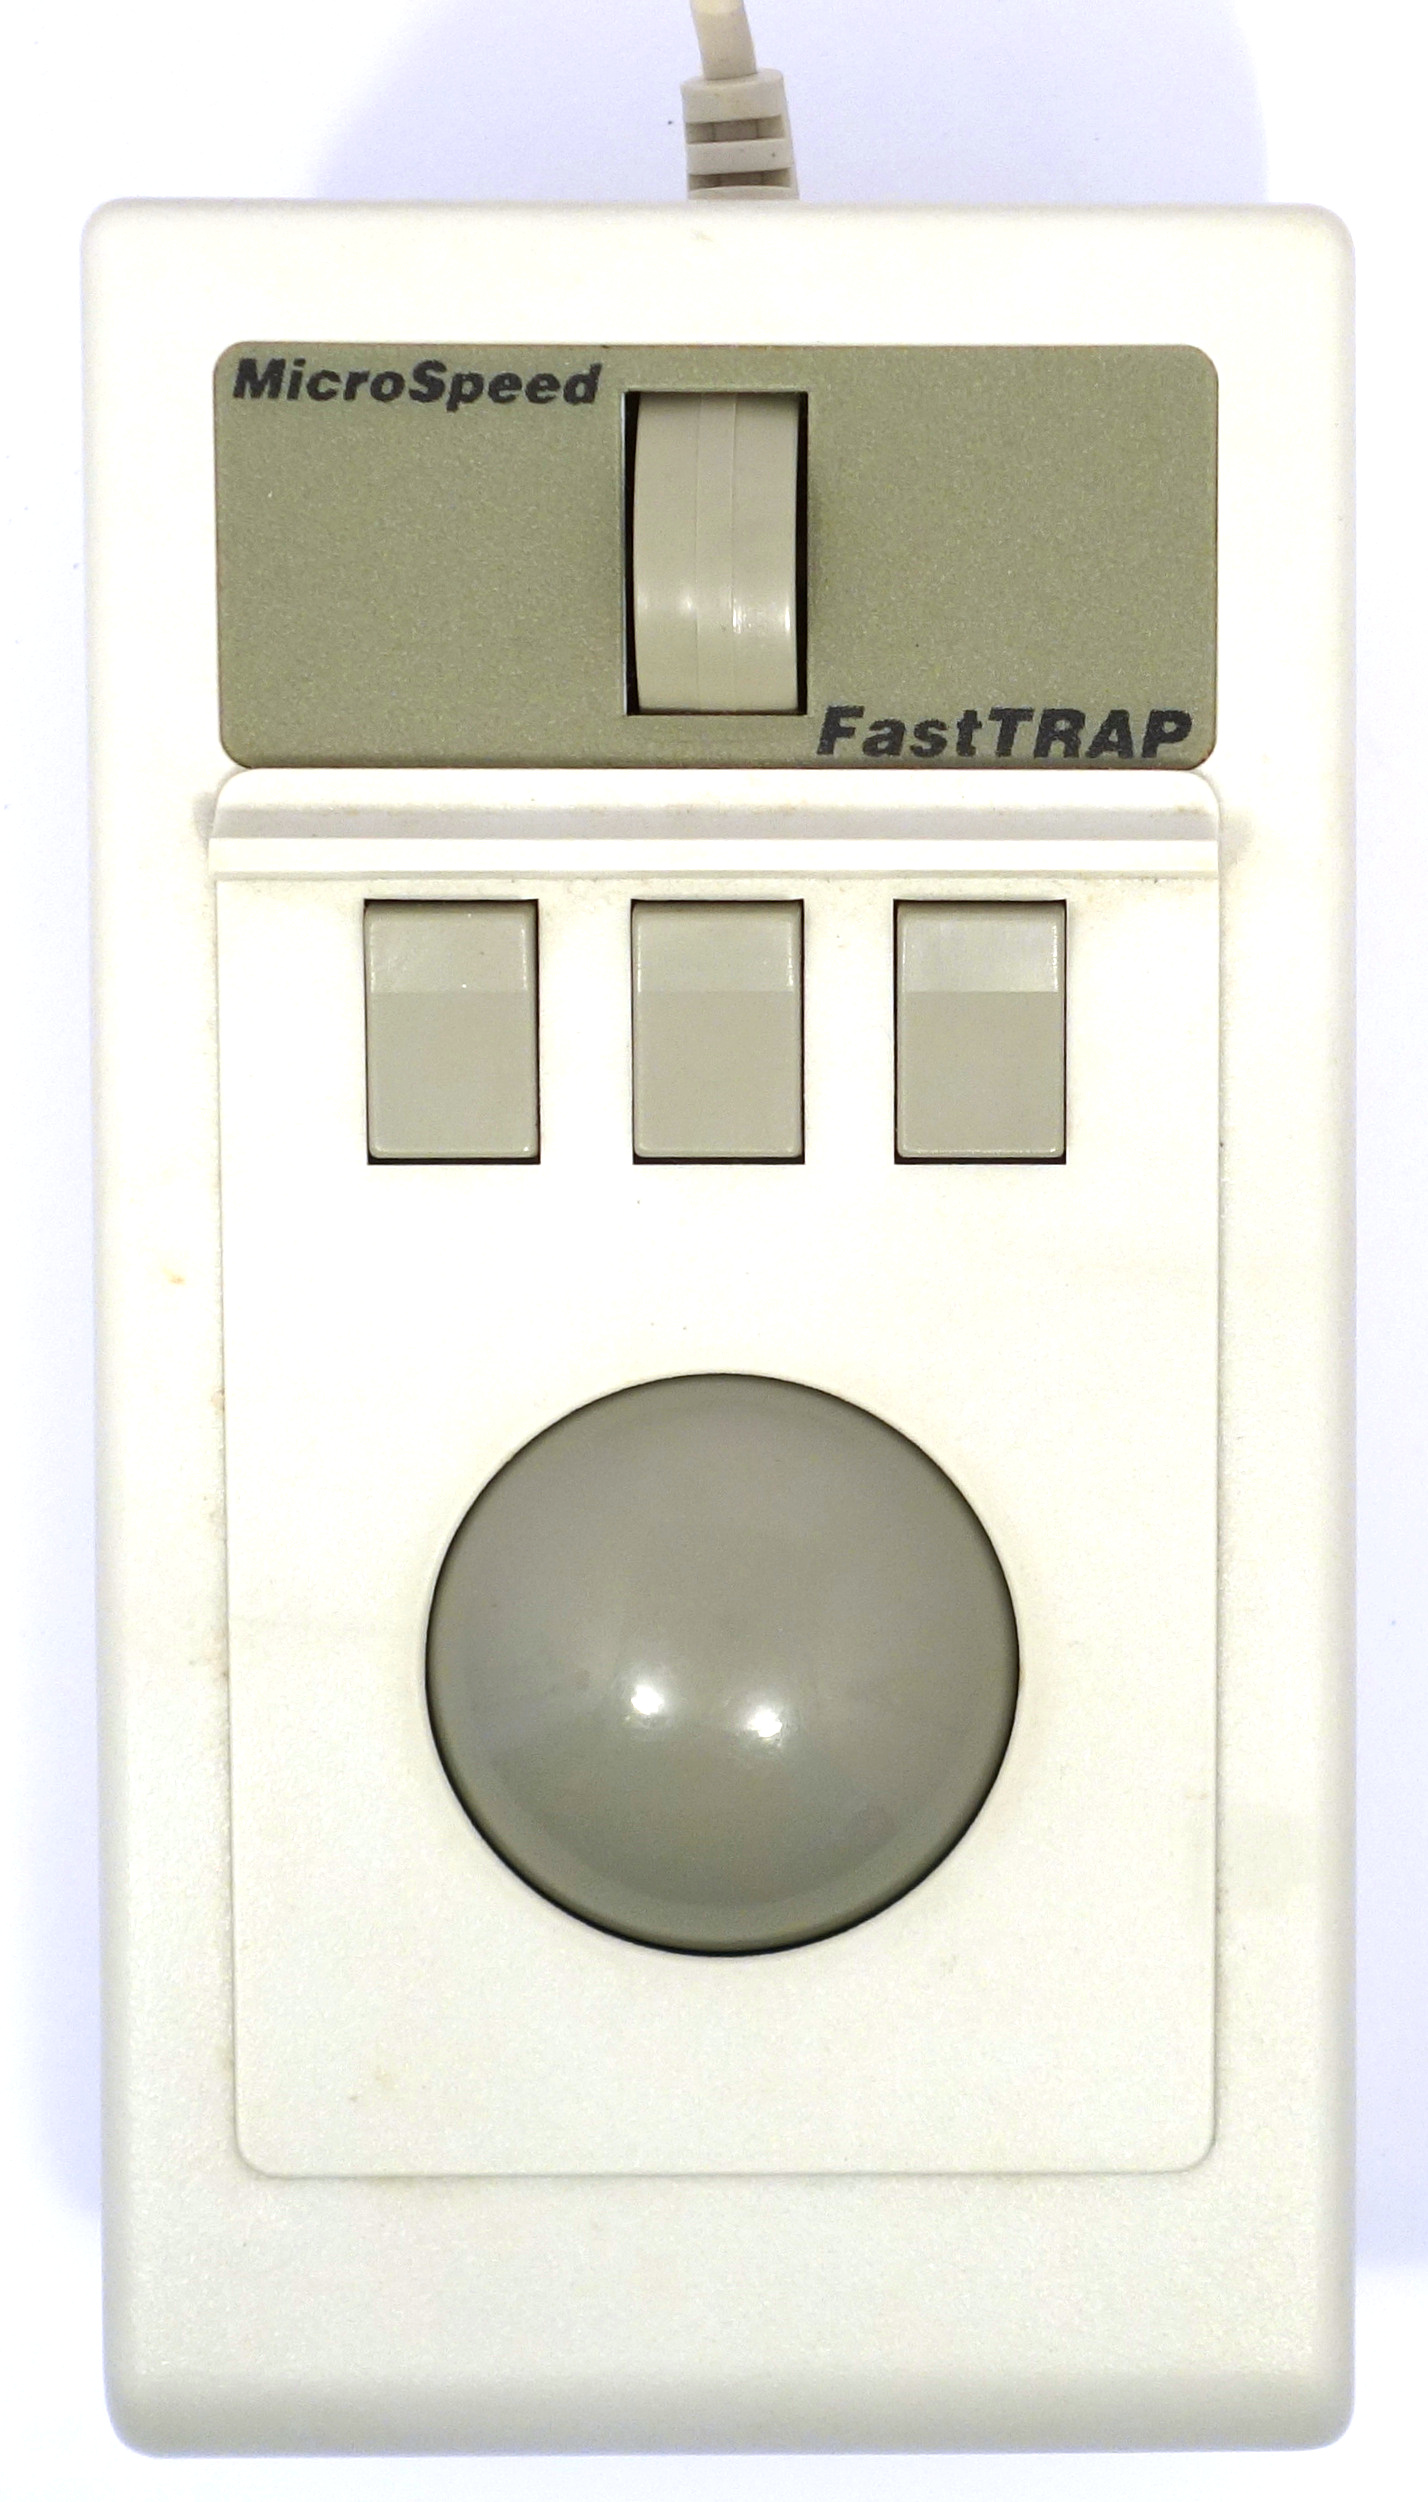
\includegraphics[scale=0.3]{1987_microspeed_fasttrap/top_60.jpg}
    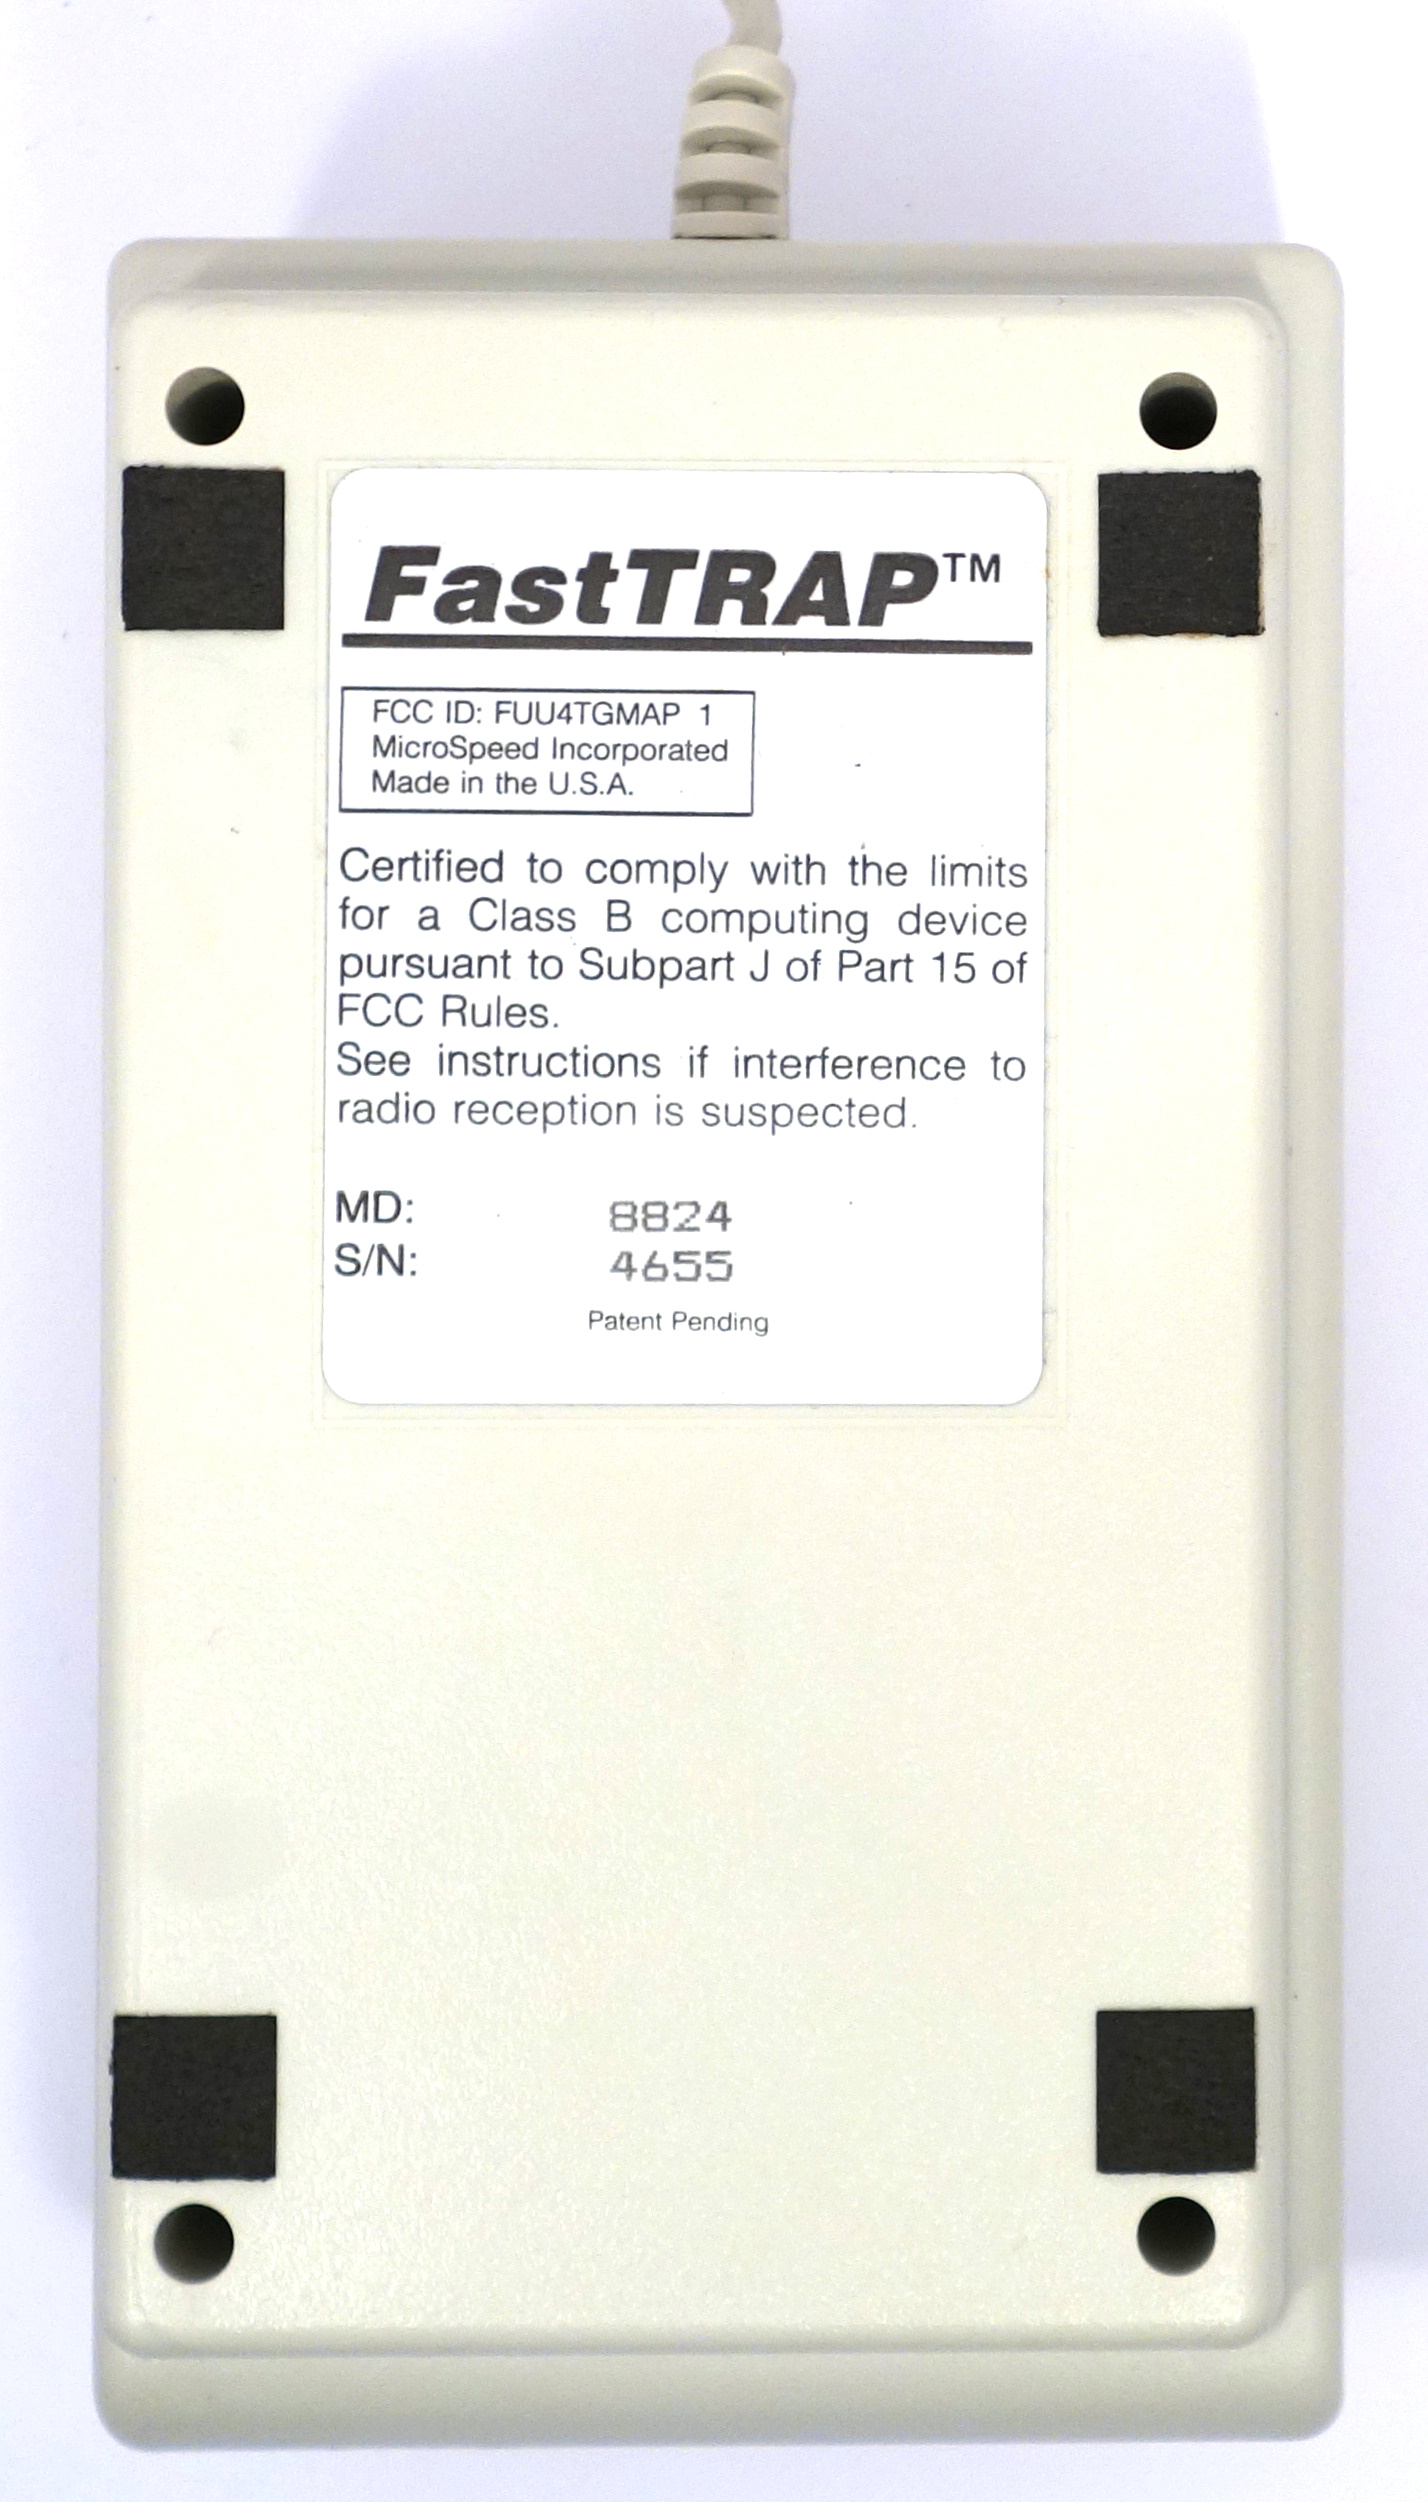
\includegraphics[scale=0.3]{1987_microspeed_fasttrap/bottom_60.jpg}
    \caption{FastTRAP, top and bottom views}
    \label{fig:FastTRAPTop}
\end{figure}

When connected to a computer, FastTRAP uses the Microsoft mouse protocol and can use the appropriate standard driver. The specialized driver included in the kit is required only for working with the third coordinate. The configuration software also allows you to reprogram the functions of the keys, the ball and the wheel, allowing you to adapt the device to any software: for example, execute certain DOS commands  \cite{fast}.

\begin{figure}[h]
   \centering
    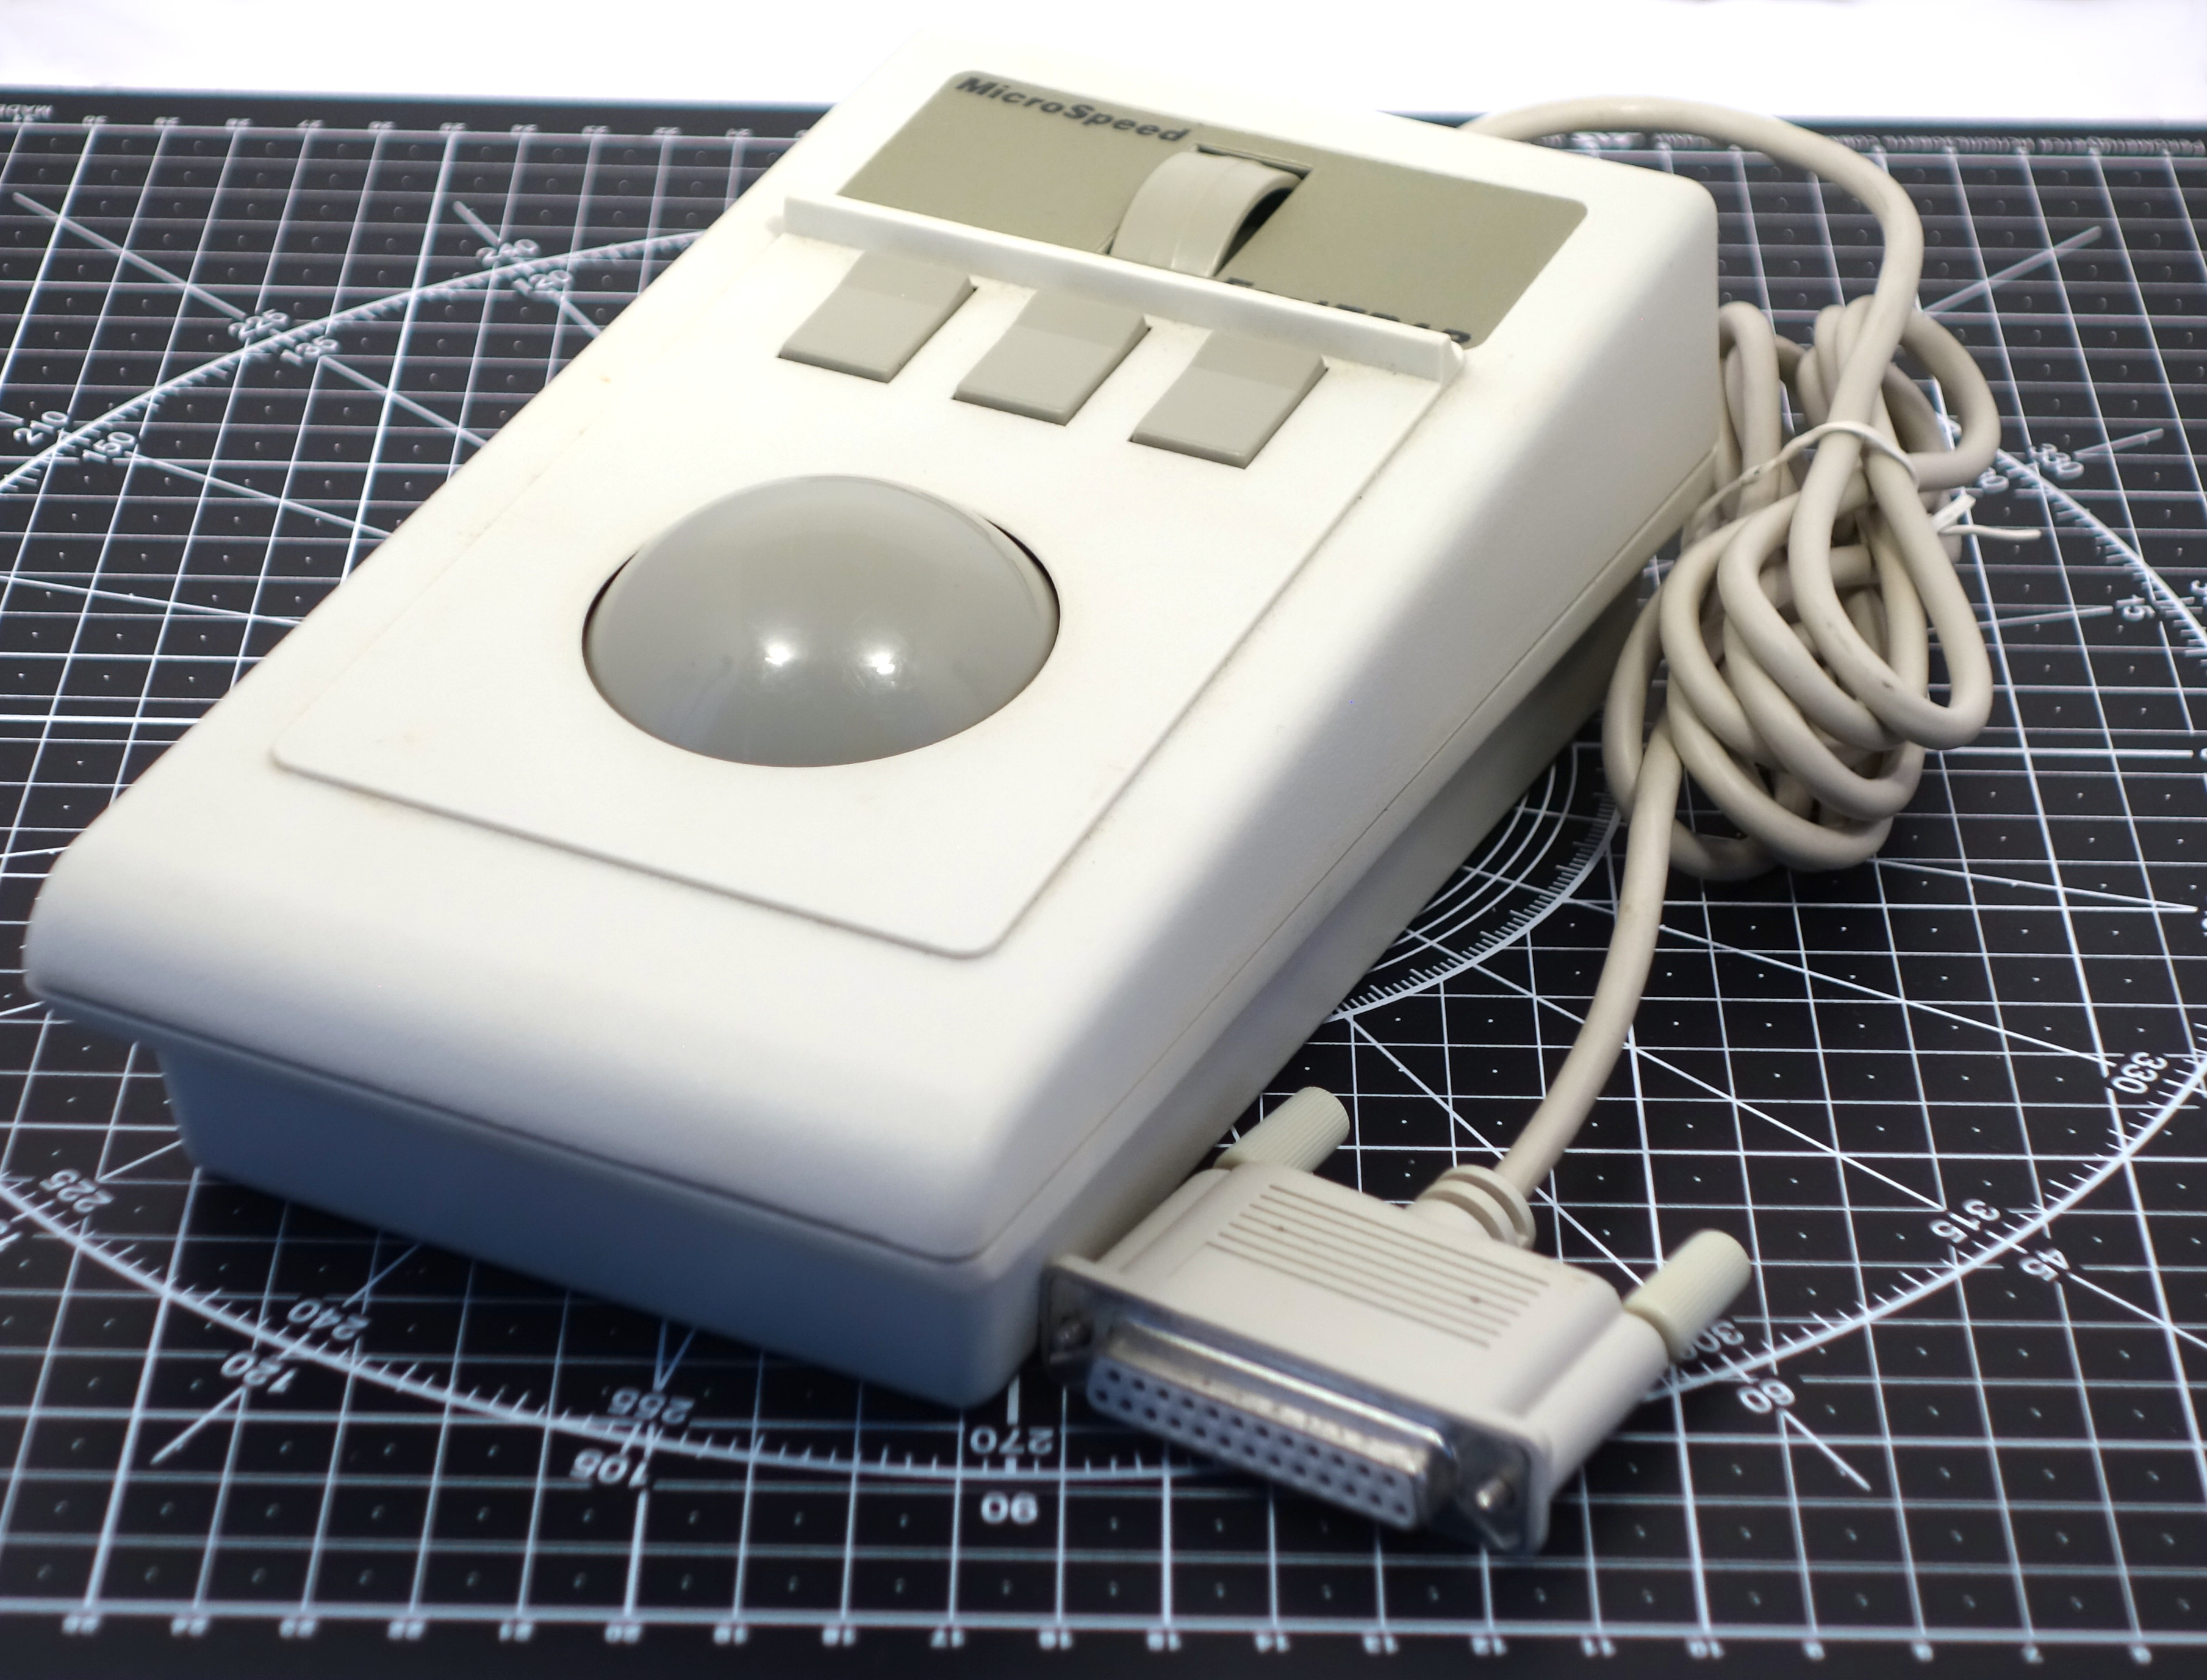
\includegraphics[scale=0.4]{1987_microspeed_fasttrap/size_15.jpg}
    \caption{FastTRAP on a graduated pad with a grid step of 1~cm}
    \label{fig:FastTRAPSize}
\end{figure}

The trackball is very large (figure \ref{fig:FastTRAPSize}, \ref{fig:FastTRAPHand}). In addition to the third coordinate, FastTRAP gives CAD users the advantage of a large ball: accurately moving the cursor in the graphics window is easier than moving the mouse to the desired position (and sometimes you can't avoid accidentally moving the mouse when pressing a button).

\begin{figure}[h]
    \centering
    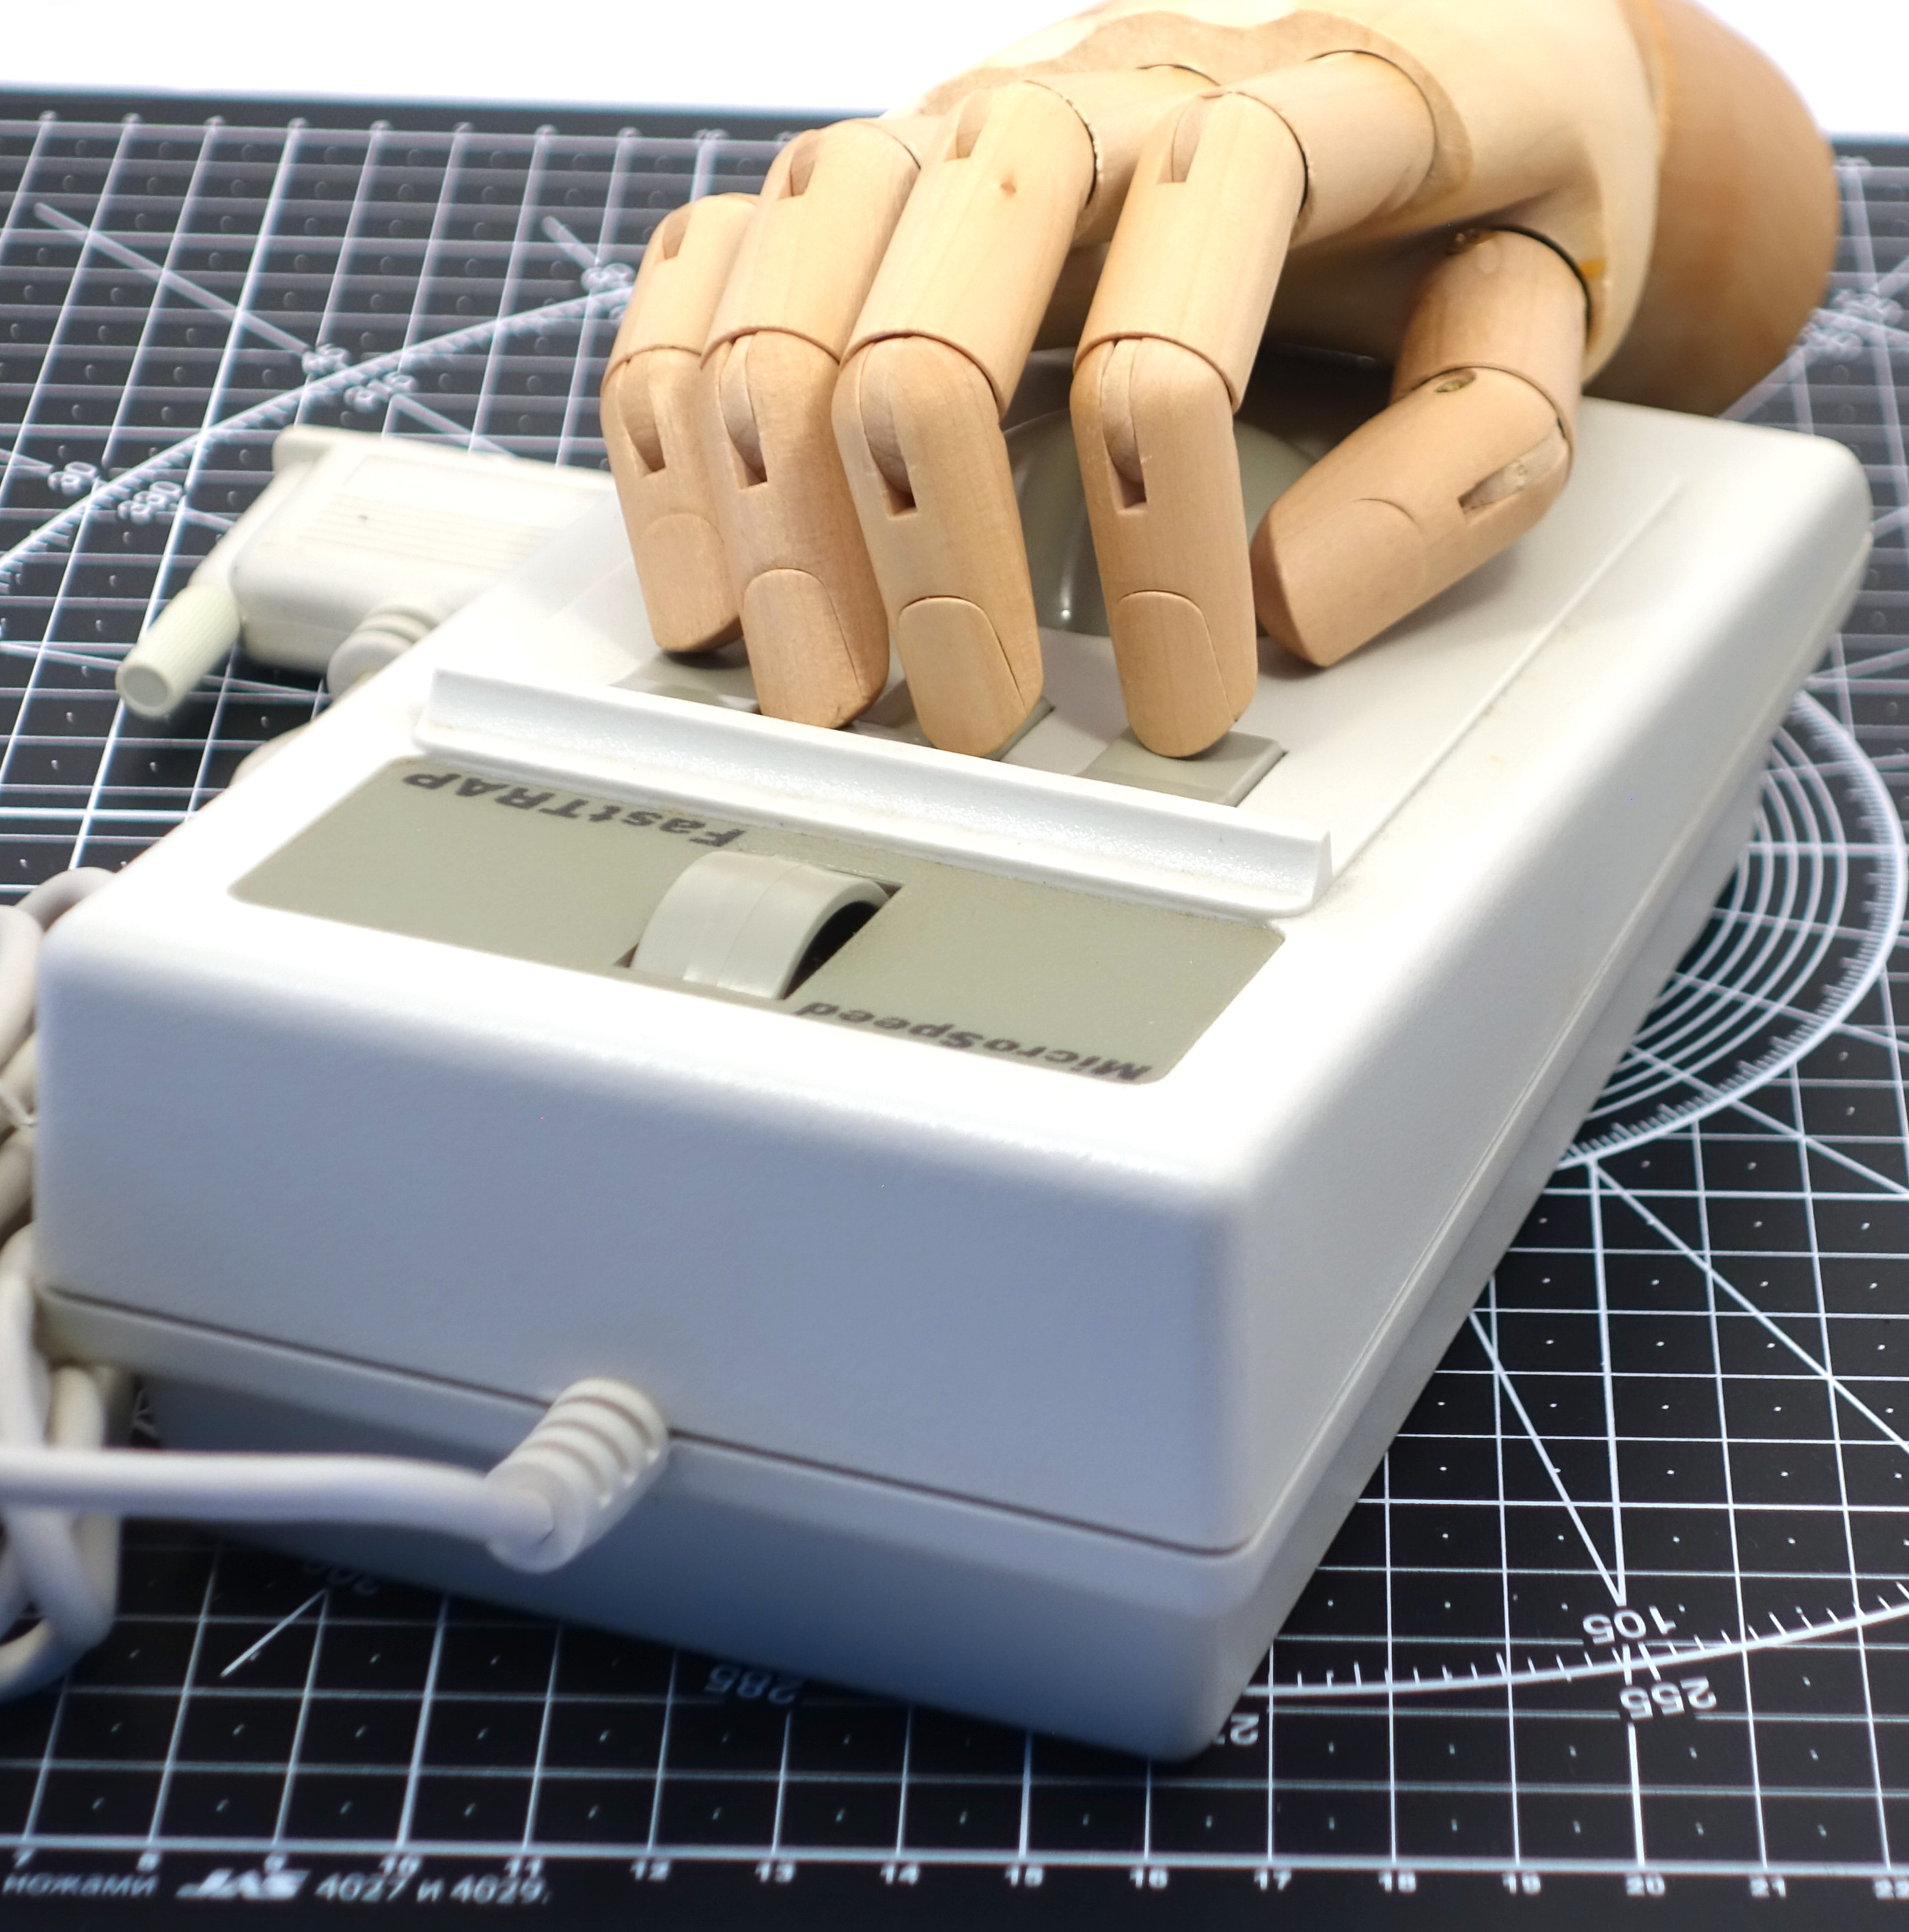
\includegraphics[scale=0.3]{1987_microspeed_fasttrap/hand_15.jpg}
    \caption{FastTRAP with a human hand model}
    \label{fig:FastTRAPHand}
\end{figure}

In terms of ergonomics, the trackball buttons are well positioned for easy reach when the user's palm covers the ball. However, the wheel is on the farthest edge of the body from the user, and it may be necessary to move the hand to rotate it (figure {fig:FastTRAPTop}, \ref{fig:FastTRAPHand}).


\begin{figure}[h]
    \centering
    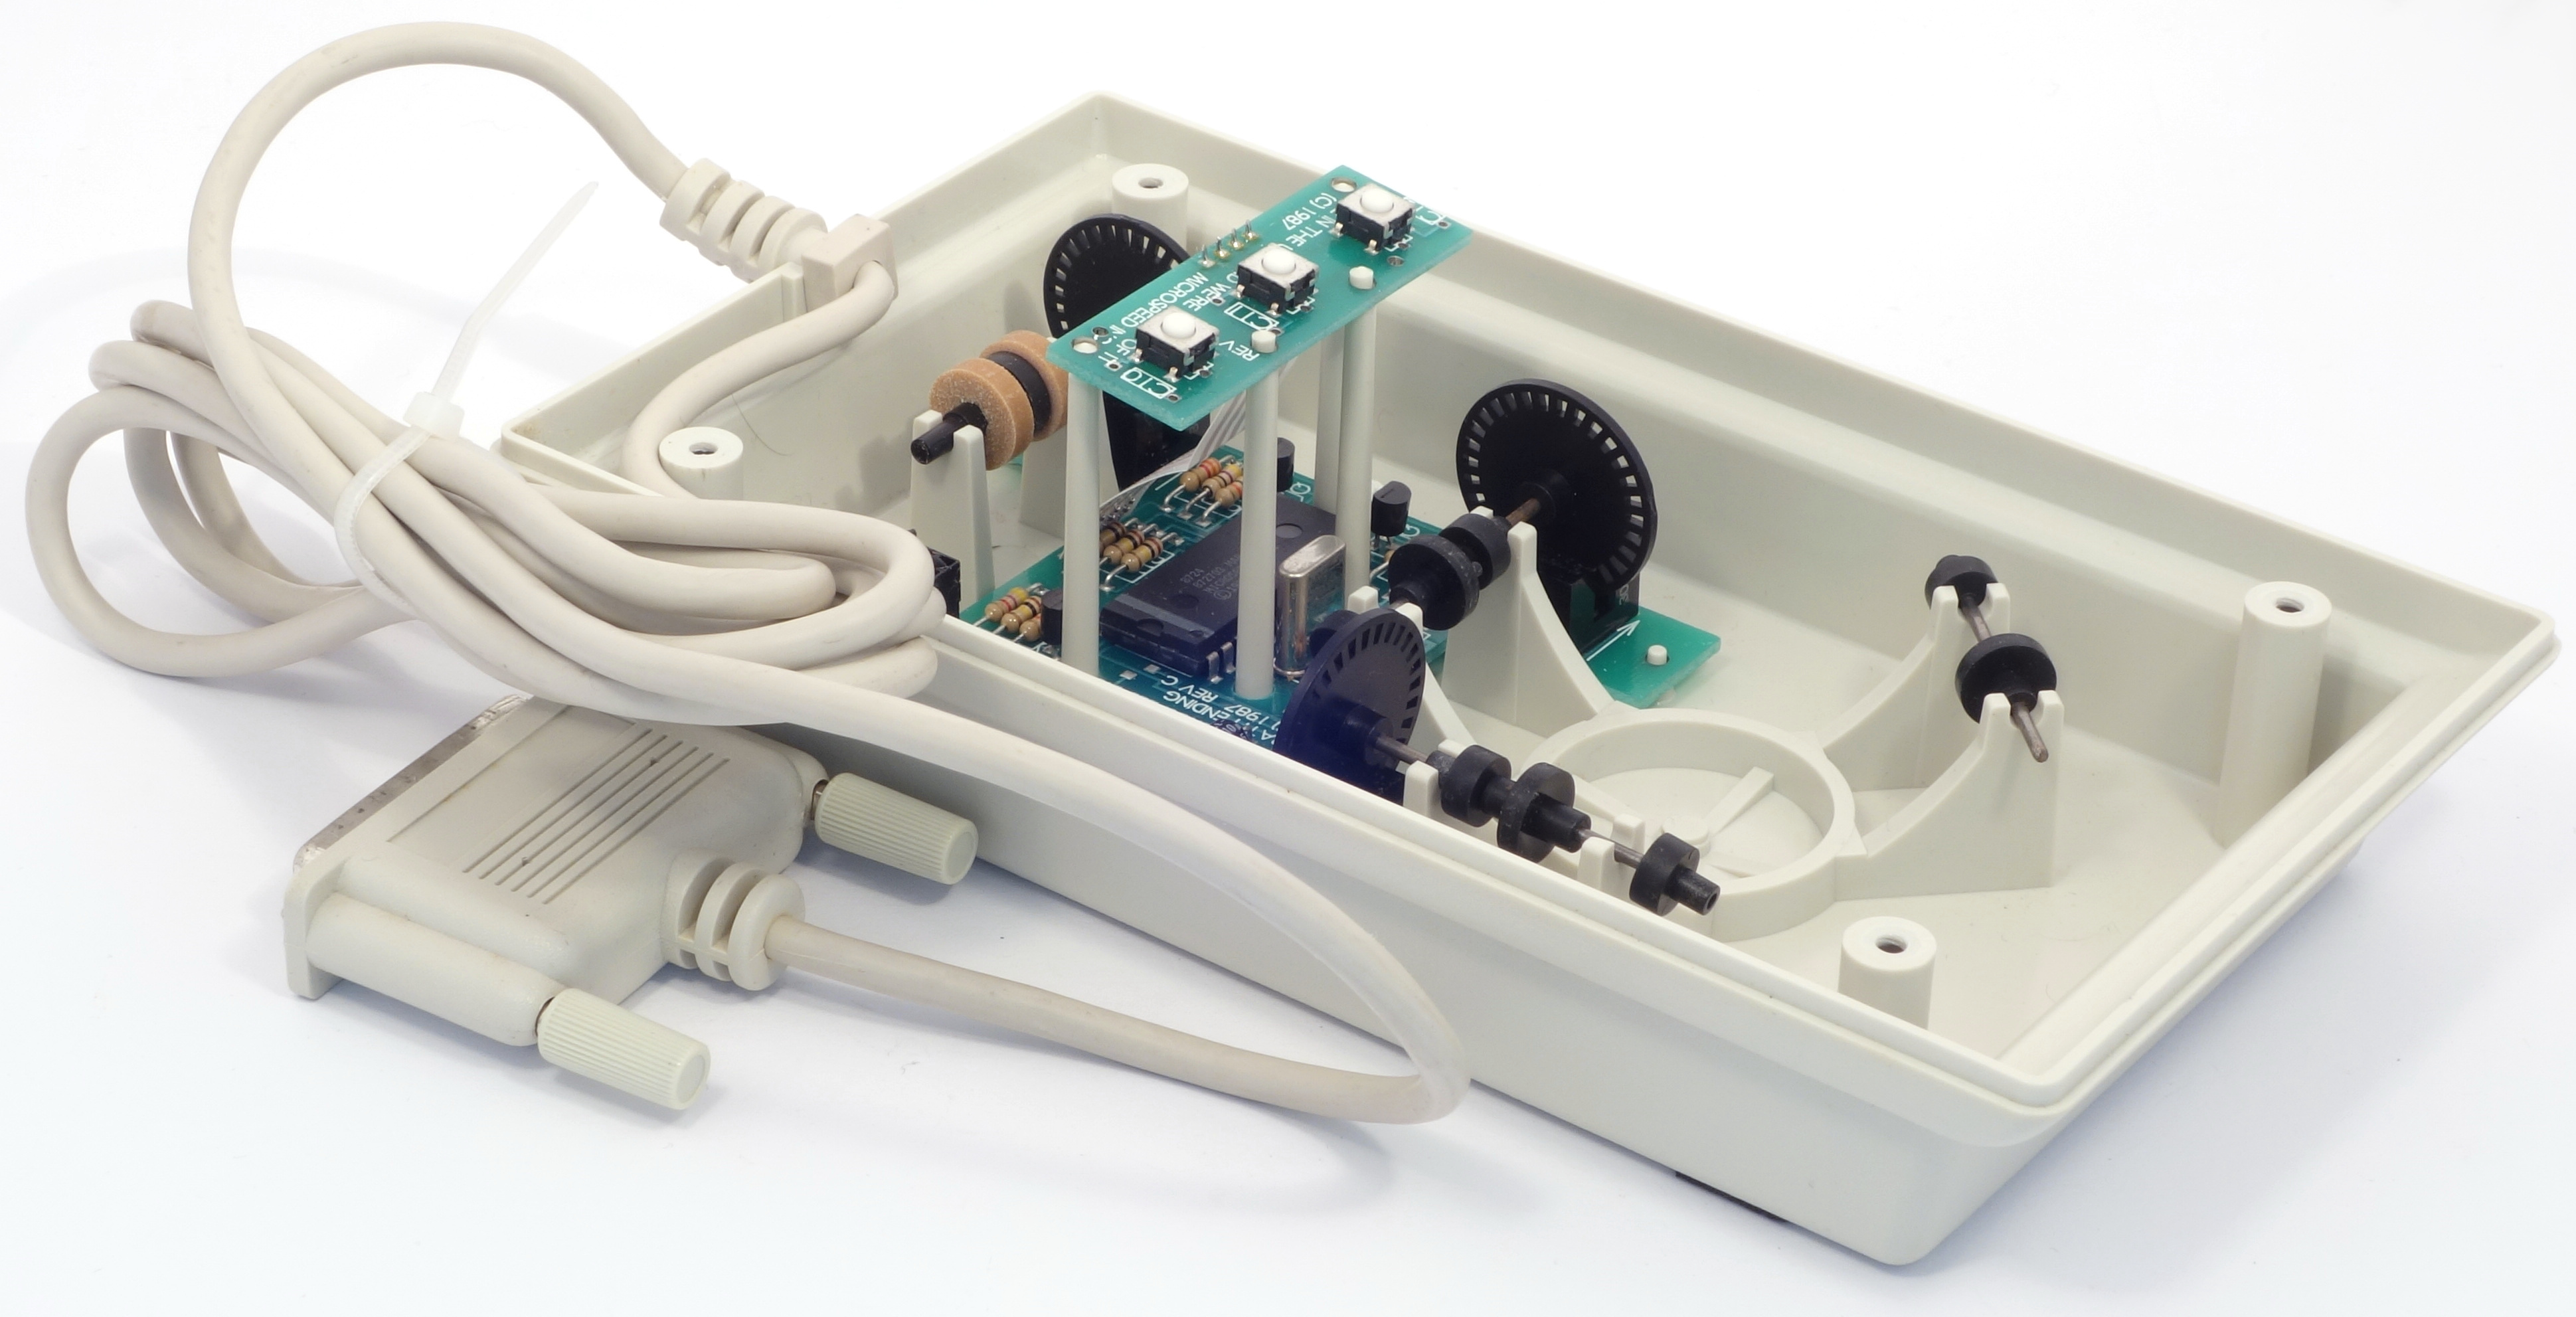
\includegraphics[scale=0.6]{1987_microspeed_fasttrap/inside_15.jpg}
    \caption{FastTRAP disassembled}
    \label{fig:FastTRAPInside}
\end{figure}

Trackball internals are shown on figure \ref{fig:FastTRAPInside}. The standard optomechanical design is supplemented by frictional gear connecting a roller with an additional optomechanical encoder. It can also be noted that the encoders used to measure the movement along all three axes are the same: on the one hand, this was not the most difficult task in terms of layout (taking into account the large size of the case), but on the other, it can be quite appropriate, given the purpose of the additional wheel.

\begin{thebibliography}{9}
\bibitem {fast} G. Kunkel. The 3-D FastTRAP points with precision // PC Magazine, November 24, 19987. - p. 56.
\end{thebibliography}
\end{document}
